\chapter{\textsc{IACS cyber range design}} \label{ch:cr-design}

This chapter concentrates on the design of CR for use in offensive capability development exercises and, in a structured manner, introduces and explores various aspects of IACS CR development and design considerations. 

\section{Overview}

The author has designed the IACS CR taking into account identified gaps from section \ref{sec:identified-gaps}, additional literature reviews about IACS vulnerabilities, and the author's personal practical experience in the IACS field as he has done testing, implementation, and configuration of various IACS components in the past.

This master thesis objective is to create the CR by utilizing key aspects from the literature review (see Sec. \ref{sec:novel-contrib}). Developed IACS cyber range encompasses the following characteristics:

\begin{itemize}
	\item realistic;
	\item easily reproducible;
	\item with publicly available documentation;
	\item supporting multistage attack scenarios;
	\item oriented to use in offensive exercises (see Sec. \ref{subsec:offensive-ops}).
\end{itemize}

Since most of the population nowadays is concentrated around the cities, it is crucial to sustain this population by providing water, electricity, heating, transportation, communication, and several other services. Most infrastructures are controlled and automated by the IACS, and any interruption or loss of these services is likely to have a devastating effect.

For this CR, as a primary physical process, the district heating plant is used. The district heating plant supplies heat to the city. A secondary control process is a warehouse management system controlling alarms and lights. The warehouse is part of the heating plant and is used to store materials, spare parts, and other goods necessary to ensure continuity of heating plant operation. The heating plant and warehouse are collocated, and as seen in figure \ref{fig:cr-network-topology} they are connected in one communication network. The author has chosen the heating plant as it is part of the critical infrastructure for the cities, and they can be valuable targets for adversaries. The second reason is that the heating process is relatively easy to comprehend and understand the causality of different physical mechanics.

The CR network topology is shown in figure \ref{fig:cr-network-topology}. The system consists of two PLCs (3) and (4), SCADA (2) and WEB-SCADA (1). So CR can be divided into supervisory and control systems containing SCADAs, and execution systems containing PLCs. Further, each of the elements, working principles, communication, and simulated physical systems are described in detail.

Author’s choice of elements was motivated by two reasons. Firstly, as indicated in the literature review, CR should encompass elements used in the target region. Europe is the target region for this master thesis. In Europe, Siemens is one of the vendors widely used across various IACS industries. Moreover, as the cost of physical devices is not negligible and the master thesis was performed without any budget, the author used  Siemens equipment already accessible from other projects. Table \ref{tab:cr-el-list-2} describes the hardware and software of each element, used versions, and Siemens reference code for respective devices. In further sections, each of these elements, purpose, and communication partners are described in detail.

\begin{figure}[htb]
	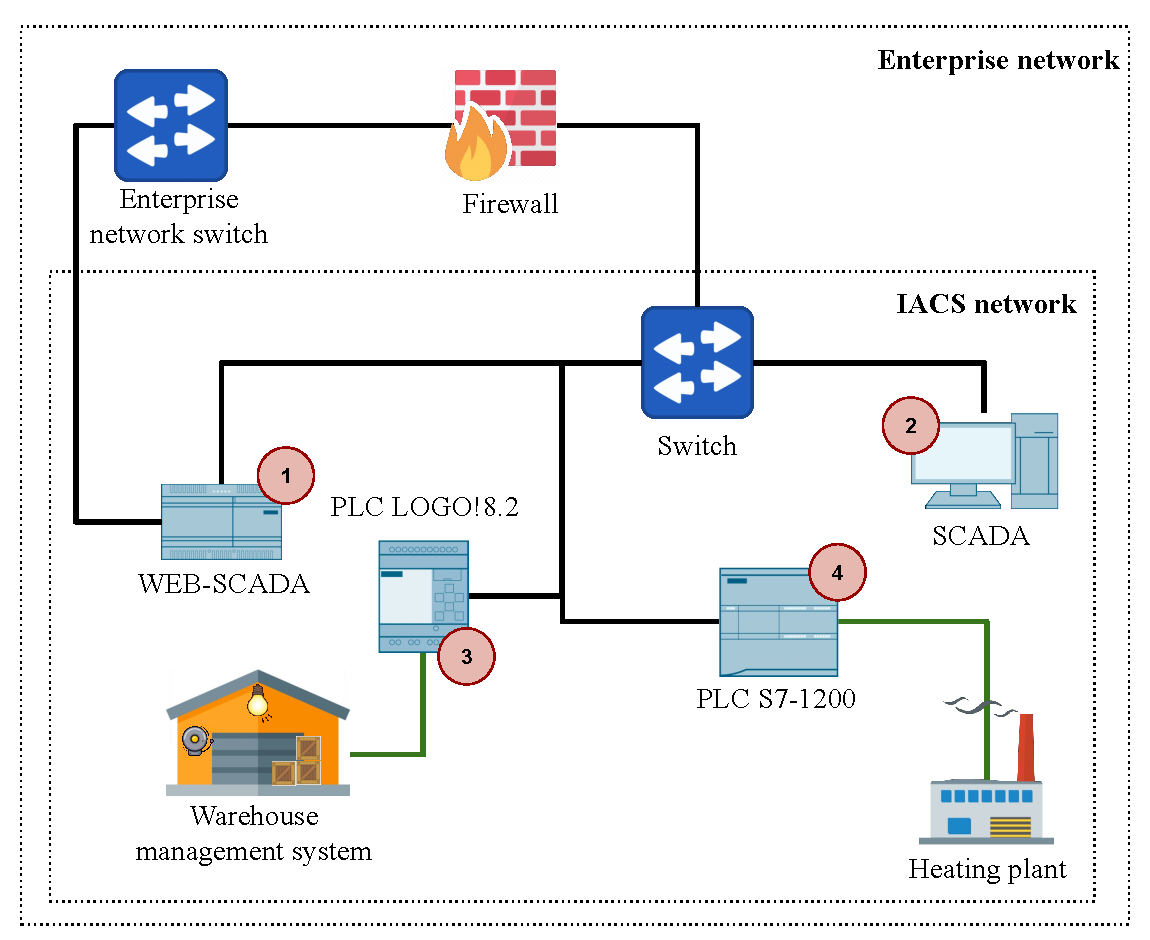
\includegraphics[width=\linewidth]{rangeX-CR-no-attacker.pdf}
	\caption{The CR network topology created by the author.}
	\label{fig:cr-network-topology}
\end{figure} 


\begin{longtable}[htb]{|c|c|p{0.35\textwidth}|p{0.3\textwidth}|}
	\caption{\raggedright{List of elements and their system description used in CR.}}
	\label{tab:cr-el-list-2}\\
	\hline
	\textbf{Nr.}       & \textbf{Element}           & \textbf{System description}                                                                                                                            & \textbf{Siemens reference} \\ \hline
	\endhead
	%
	\multirow{3}{*}{1} & \multirow{3}{*}{SCADA}     & Siemens, Simatic WinCC Advanced   V15.1                                                                                                                & 6AV2102-0AA05-0AA5       \\ \cline{3-4} 
	&                            & MS Windows 7 enterprise, SP1, Build 7601                                                                                                                & n/a                      \\ \cline{3-4} 
	&                            & VirtualBox   V6.0                                                                                                                                      & n/a                      \\ \hline
	\multirow{3}{*}{2} & \multirow{3}{*}{WEB-SCADA} & NodeRed V1.0.0 \footnote{NodeRed   - (\url{https://nodered.org/}) } & n/a                      \\ \cline{3-4} 
	&                            & Yocta   Linux V2.6                                                                                                                                     & n/a                      \\ \cline{3-4} 
	&                            & IOT2040                                                                                                                                                & 6ES7647-0AA00-1YA2       \\ \hline
	2                  & PLC LOGO!                  & Siemens, LOGO! 8.2, Full   versions: 1.82.02                                                                                                           & 6ED1052-1FB08-0BA0       \\ \hline
	3                  & PLC S7-1200                & Siemens, Simatic S7-1200, CPU   1215C                                                                                                                  & 6ES7215-1AG40-0XB0       \\ \hline
\end{longtable}

\section{Heating process} \label{sec:heat-proces}


SCADA HMI visualization of the heating plant is shown in figure \ref{fig:scada-heating-view}. The heating plant consists of:

\begin{itemize}
	\item Heating transmission line - transports \gls*{htf} to the city;
	\item Circulation pump (A1) - forces the HTF flow to the city;
	\item Transmission line valve (A3) - required to be open for the \gls*{htf} to circulate;
	\item Gas flow valve (A2) - control the burning temperature of the gas in the burning chamber;
	\item Temperature and pressure sensors (S3, S4) - to monitor and give feedback to the control system about temperature and pressure in HTF tank;
	\item Flow speed sensor (S1) - To monitor and give feedback to the control system about the state of the HTF flow speed.
\end{itemize}

\begin{figure}[htb]
	\centering
	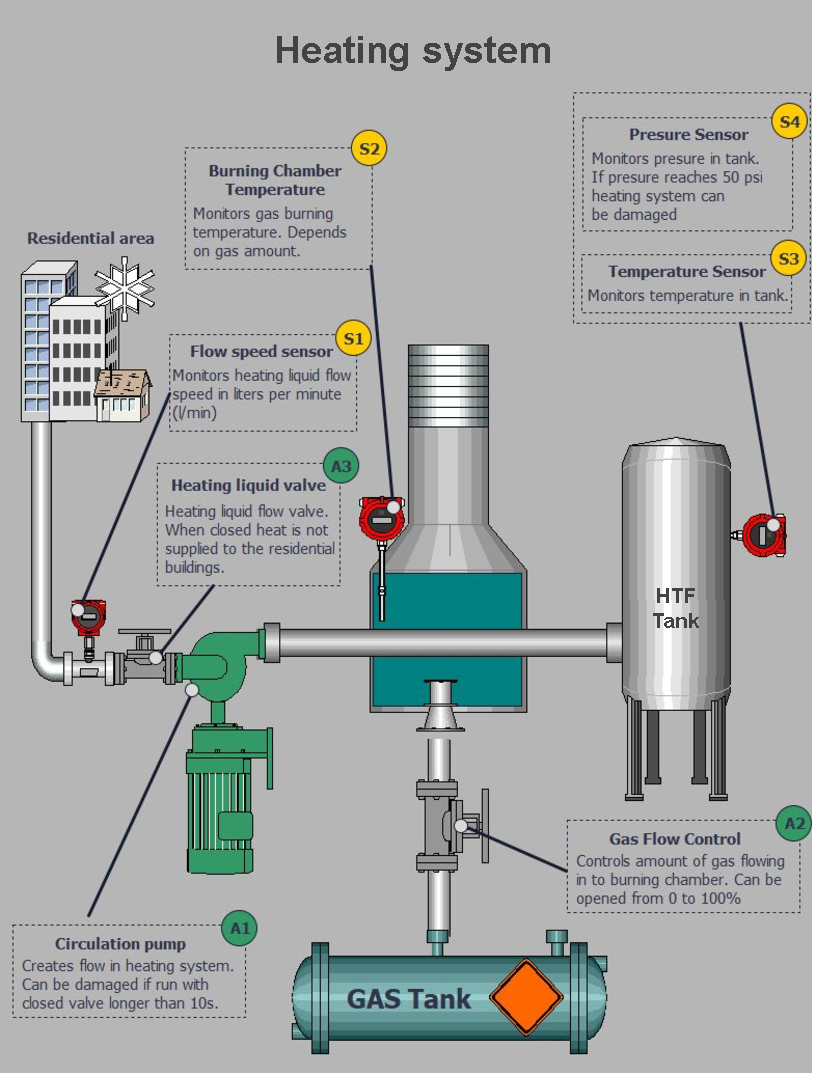
\includegraphics[height=0.58\textheight, keepaspectratio]{SCADA-heating-system-with-design-small.pdf}
	\caption{The heating plant visualization created by the author.}
	\label{fig:scada-heating-view}
\end{figure}

The heating process can be divided into two phases. One of the phases is the heating of HTF, and the second is HTF transmission to the city districts:

\begin{enumerate}
	\item HTF is heated by burning gas in the furnace. Then the heated fluid is distributed to the rural area. Gas flow is related to the burning temperature. Burning temperature is controlled by gas flow valve A2 (see Fig. \ref{fig:scada-heating-view}). To automate the burning process, an operator sets a setpoint with the desired fluid temperature level. S7-1200 PLC (see Fig. \ref{fig:cr-network-topology}) compares setpoint temperature with the actual heat transfer fluid temperature S4. Based on that, S7-1200 PLC controls gas-burning temperature S2  by adjusting gas flow controller A2. This system has embedded physical limits, such as, maximum temperature and maximum pressure. After exceeding maximum values, the heating plant gets damaged. If temperature or pressure values reach a set threshold, S7-1200 automation protects  the physical system by stopping the gas flow to safeguard against the damage;
	
	\item The HTF transmission process depends on the heating process. When HTF in the transmission line reaches temperature 60° C, then circulation pump A1 switches on, and heating valve A3 opens. In this phase heating system is fully operational, and heat is delivered to the city districts. However, this part of the system can be damaged irreversibly if the circulation pump runs with the heating liquid valve (A3) closed.
\end{enumerate}

Heating process control logic is in PLC S7-1200 (see Fig. \ref{fig:cr-network-topology}). The author has built CR to be easily reproducible with no additional hardware, sensors, or actuators attached to S7-1200. Instead, the physical process is simulated using the \gls*{hil} method. HIL consists of a simplified mathematical model of the heating process. HIL includes and controls nominal values of the physical process so that it can be damaged if these values exceed, which means that both the control program and HIL program runs on the same device. Both programs are separated so that control logic can only interact with heating process simulation as if through sensors and actuators seen in figure \ref{fig:scada-heating-view}. For this reason, part of the controller responsible for physical system simulation is off-limits for the CR participants.

S7-1200 is Siemens Simatic PLC, which is widely utilized in different industrial fields. This PLC can have multiple configurations by adding expansion blocks like additional I/O ports, additional communication interfaces, and process-specific extensions. In this CR, basic S7-1200 module is used with built-in I/O and communication ports (see Tab. \ref{tab:cr-element-com}).

S7-1200 was configured and programmed utilizing Siemens software TIA Portal advanced V15.1 \footnote{TIAportal -  \url{https://new.siemens.com/global/en/products/automation/industry-software/automation-software/tia-portal.html} }. The TIA Portal is a multipurpose platform that allows the programming and configuration of Simatic PLC and other peripheral devices like networking components, HMIs, and SCADAs. TIA Portal also allows access to the devices in online mode and diagnoses them during commissioning. TIA Portal supports all programming IEC61131-3 \parencite{WEB-14-plc-languages} standardized languages. Author uses LAD and SCL for this project as these languages are best suited for this program. There is no difference in using one or another language according to the author's knowledge and researched literature from the point of vulnerabilities. 

Figure \ref{fig:tia-functions} displays overall structure of S7-1200 program. For Siemens PLC most fundamental programming construct is \gls*{ob}. OBs are the highest-level constructs that are executed cyclically or by some trigger event. Research \parencite{12-ICS-testbed} states that OBs are similar to function calls in the C programming language or system calls in Unix OS. OB is always present in Simatic PLC programs and is identified as OB1. OB1 is also seen in the author's program structure in figure \ref{fig:tia-functions}. There the OB1 is used as a program's entry point where all other program functions are called. OB1 is executed cyclically as PLC's inputs and outputs (I/O) must always be updated. During the cycle, OB1 checks I/O, makes function calls and manages memory. Additionally, Simatic PLCs has a construct called \gls*{db}. DB contains global retentive variables which can be used in OB, \gls*{function}, or \gls*{fb}.

The program is structured in two parts. The first contains control functions, and the second has physical simulation functions. Information transfer between these two program parts is done by using functions \textit{actuator\_translation[FC14] and sensor\_translation[FC13]}. These two functions during each cycle copies simulated physical state:
\begin{itemize}
	\item Sensor data - from \textit{physical\_DB[DB1]} to \textit{sensor\_inputs[DB8]};
	\item Actuator data - from \textit{actuator\_output[DB9]} to \textit{physical\_DB[DB1]}.
\end{itemize}
TIAportal project files used in this CR are publicly available in the author's GitHub repository frostyICS \footnote{frostyICS - IACS cyber range for offensive capability development ( \url{https://github.com/austrisu/frostyICS})}.


\begin{figure}[htb]
	\centering
	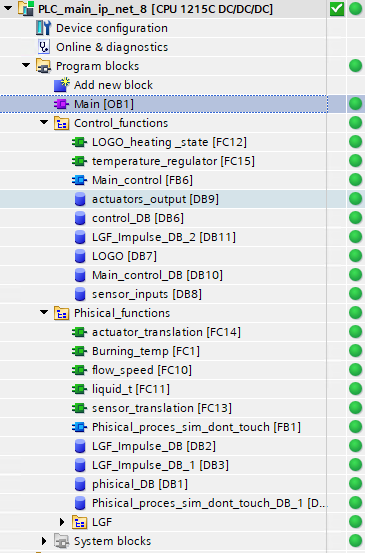
\includegraphics[height=0.52\textheight, keepaspectratio]{tia-functions.png}
	\caption{S7-1200 program structure created by the author.}
	\label{fig:tia-functions}
\end{figure}


\section{Warehouse management} \label{sec:warehouse-managment}

Warehouse management in this CR is used to control alarms and lights. This process is much simpler than the heating plant. Siemens LOGO! 8.2 PLC is used to control it as it is meant for simple applications. LOGO! can have different configurations depending on added functional modules. In this CR LOGO! 8.2 basic module (see Tab. \ref{tab:cr-element-com}) is used with built-in I/O and communication interface.

Siemens LOGO! supports two programming languages FBD and LAD. For this CR author uses FBD as this programing language is easier to comprehend. Used LOGO! program is shown in figure \ref{fig:logo-logic}. FBD program is executed from left to right. Each block represents some function that is built-in or user-defined. For example, some built-in functions are boolean operators, timers, comparators, memory write and read functions, math functions. Functions has inputs and outputs which can be connected and chained to other functions making logic instructions. For the program in LOGO! only built-in functions are used. Used functions in the program (see Fig. \ref{fig:logo-logic}) are as follows:

\begin{itemize}
	\item NI - network input is used to read values from local LOGO! memory or to read values from other devices in the network supporting S7comm protocol;
	\item NQ - network output is used to write values to local LOGO! memory or to write values to other devices on a network supporting S7comm protocol;
	\item Q - output is used to control LOGO! physical digital inputs and outputs (I/O);
	\item hi - keeps function output always in high state;
	\item B001 - display function is used to configure what information is displayed on LOGO! built-in screen.
\end{itemize}

LOGO! stores variables in several address types. Each address type is used for a specific purpose listed in table \ref{tab:logo-mem-spaces}. In this program, Q and V address types are used. V address type is used so that Modbus can interact with the LOGO! program. Q is used so that the program can control LOGO! 8.2 physical outputs.

\begin{longtable}[c]{|l|c|c|c|}
	\caption{\raggedright{LOGO! 8.2 used address types (R- read, W-write).}}
	\label{tab:logo-mem-spaces}\\
	\hline
	\textbf{Address   Type}  & \textbf{Range} & \textbf{Direction} & \textbf{Unit} \\ \hline
	\endhead
	%
	Inputs (I)               & 1 – 24         & R                  & bit           \\ \hline
	Outputs (Q)              & 1 – 20         & R/W                & bit           \\ \hline
	Marker bit (M)           & 1 – 64         & R/W                & bit           \\ \hline
	Data block 1 (V)         & 0.0 – 850.7    & R/W                & bit           \\ \hline
	Data block 1 (VW)        & 0 – 850        & R/W                & 16 bits       \\ \hline
	Analog Input (AI)        & 1 – 8          & R                  & 16 bits       \\ \hline
	Analog output (AQ)       & 1 – 8          & R/W                & 16 bits       \\ \hline
	Analog marker bytes (AM) & 1 – 64         & R/W                & 16 bits       \\ \hline
\end{longtable}

Siemens LOGO! program (see Fig. \ref{fig:logo-logic}) is divided into four parts: 1) light control, 2) alarm control, 3) state of heating plant, and 4) the part which enables LOGO! hardware display. For example, light control flow works as follows: 

\begin{itemize}
	\item NI1 function each cycle reads value (true or false) from bit memory space V10.1;
	\item Value from NI1 is transferred to the input of function NQ1 and Q1;
	\item NQ1 function writes value from input to memory space V33.0;
	\item Q1 function writes value from function input to LOGO! physical output, setting voltage to high or low.
\end{itemize}

\begin{figure}[htb]
	\centering
	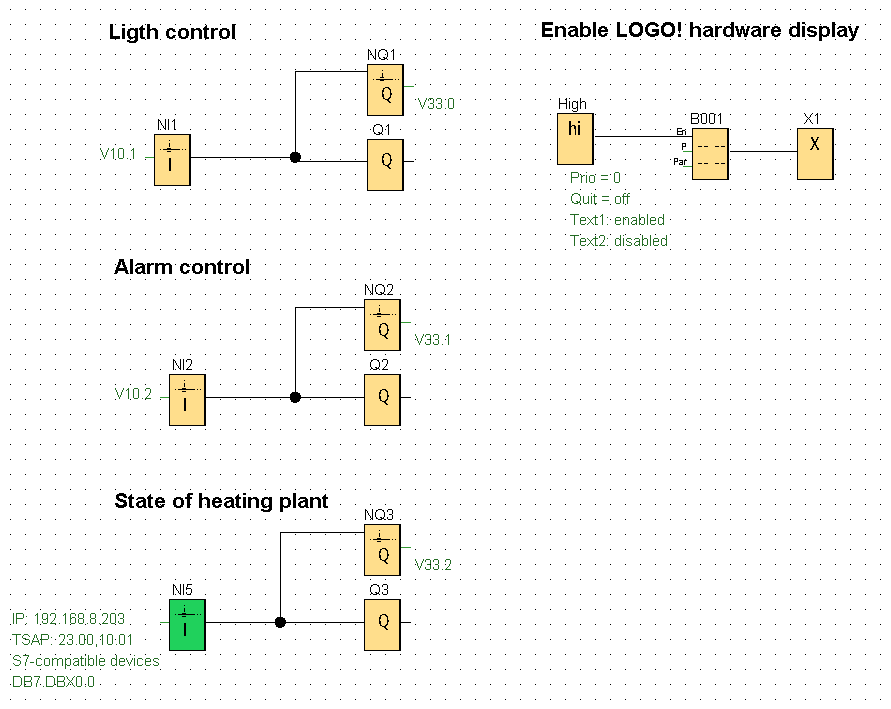
\includegraphics[height=0.42\textheight, keepaspectratio]{logo-logic.png}
	\caption{Siemens LOGO! program created by the author.}
	\label{fig:logo-logic}
\end{figure}

Siemens LOGO! is programmed utilizing Siemens LOGO! Soft Comfort \footnote{ Siemens LOGO! Soft Comfort - \url{https://new.siemens.com/global/en/products/automation/systems/industrial/plc/logo/logo-software.html}} software. LOGO! Soft Comfort is a programming tool specifically for Siemens LOGO!. This software has a user interface that allows creating and uploading software. LOGO! Soft Comfort project files used for this CR are publicly available in the author's GitHub repository frostyICS \footnote{frostyICS - IACS cyber range for offensive capability development (\url{https://github.com/austrisu/frostyICS})}.

\section{Supervision and control of systems}

Supervision and control system in the CR contains two SCADA devices (see Fig. \ref{fig:cr-network-topology}): 1) WEB-SCADA is to monitor and control the warehouse management system and display a simple indication of heat plant state, and 2) SCADA is used to control and monitor the heating plant. The following sections describe both SCADAs.

\subsection{Heating plant SCADA}

For the operator to visualize and interact with the process, SCADAs are used in this case. In this CR, SCADA can be used for an attacker to understand the state and purpose of the system. Heating plant is visualized using WinCC advanced V15.1 run-time (see Fig. \ref{fig:scada-programing-interface}). WinCC is the run-time of the HMI and SCADA system for use on MS Windows OS. WinCC software communicates with an automation system, reads a data block, displays process visualization, and allows an operator to interact with the automation system. 

\begin{figure}[h]
	\centering
	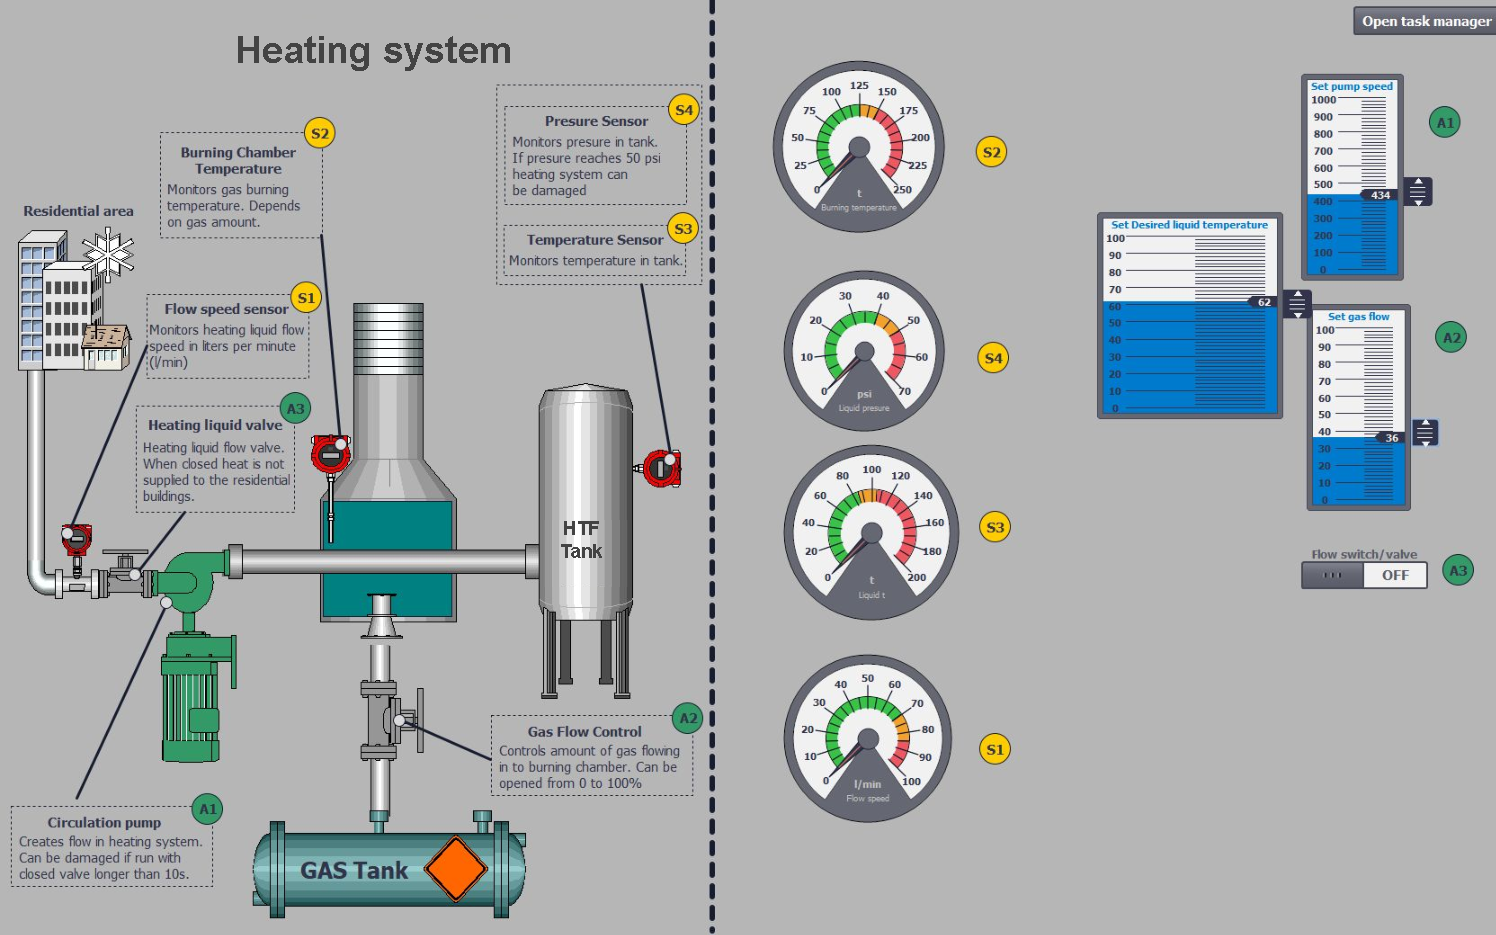
\includegraphics[width=\linewidth]{SCADA-heating-system-with-design.pdf}
	\caption{SCADA visualization screen created by the author.}
	\label{fig:scada-programing-interface}
\end{figure} 

TIA portal advanced V15.1 is used to create the WinCC application. For this CR, both S7-1200 and WinCC applications are created under the same TIA portal project because this way, communication between two applications is established. Project structure is displayed in figure \ref{fig:wincc-program}. Main parts of the application is located in folders \textit{Screens} and \textit{HMI tags}. \textit{Screens} are where visualization of heating system is created. \textit{HMI tags} are where mapping of S7-1200 and WinCC application variables, also called tags, is done. Therefore, making them available for both applications across the network. 

\begin{figure}[h]
	\centering
	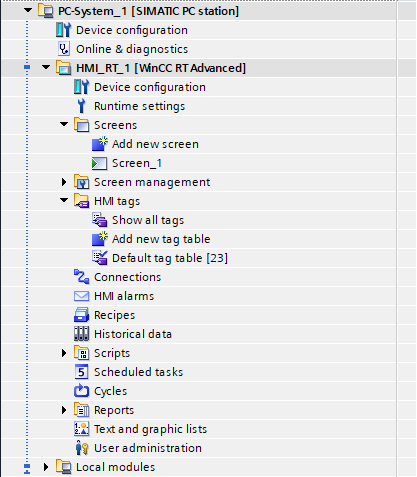
\includegraphics[height=0.42\textheight, keepaspectratio]{wincc-program.png}
	\caption{WinCC SCADA application structure created by the author.}
	\label{fig:wincc-program}
\end{figure}

\subsection{Warehouse management WEB-SCADA}

WEB-SCADA is different from conventional SCADA as it utilizes web technologies for visualization and usually can be accessible as a web page. For this CR, author utilizes web technologies such as NodeRed to create WEB-SCADA. Based on author's opinion and experience, some organizations cut corners and create simple web interfaces to control assets located in the field. Sometimes, due to a lack of budget, they create these solutions by themselves, possibly creating even more security risks. 
%Hence, this solution is used in the CR. 

Previously mentioned security gaps are the reason why for developing WEB-SCADA author chose NodeRed \footnote{NodeRed - \url{https://nodered.org/}} which is a low-code platform where programming is similar to FBD. NodeRed is suitable for simple DIY system solutions sometimes encountered in IACS. Additionally, NodeRed is used in RevolutionPI \footnote{RevolutionPI - \url{https://revolution.kunbus.com/}}, which is on RaspberryPi based PLC for industrial DIY projects. Overall, created NodeRed application communicates with LOGO! 8.2 to display and control warehouse lights and alarms. Additionally, WEB-SCADA collects and visualizes data from LOGO! about heating plant state. Visualization can be seen in figure \ref{fig:web-scada}.

\begin{figure}[H]
	\centering
	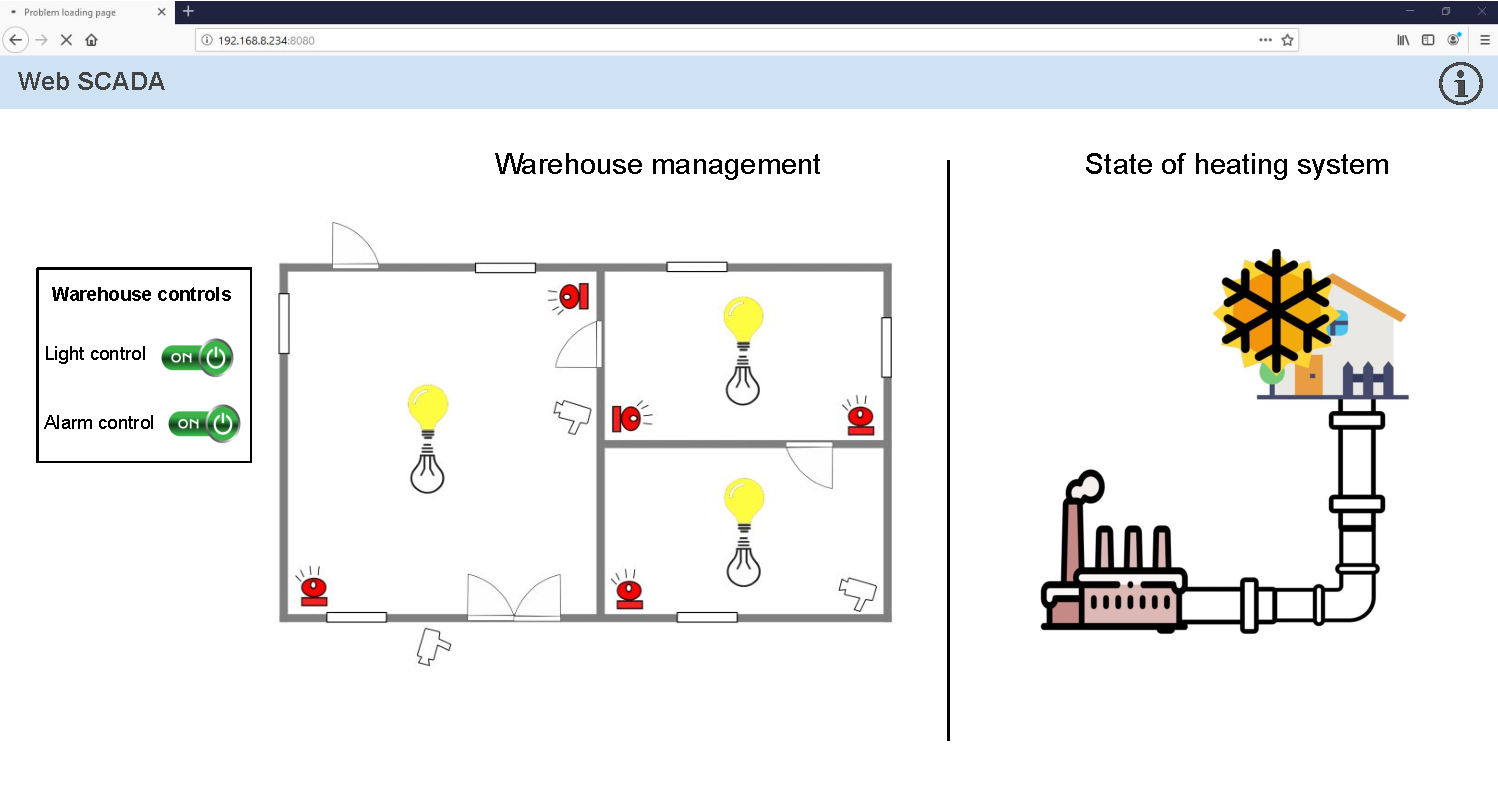
\includegraphics[width=\linewidth]{web-scada.pdf}
	\caption{Warehouse management system visualization created by the author.}
	\label{fig:web-scada}
\end{figure}

The WEB-SCADA application resides on the Siemens IOT2040 hardware, a budget industrial PC designed to withstand industrial environments. IOT2040 has two network interfaces. Hence, misconfiguration is introduced by connecting one interface directly to the enterprise network bypassing the IACS firewall (see Fig. \ref{fig:cr-network-topology}). The misconfiguration of the CR network represents an intentional or incorrect network configuration that bypasses the intended security mechanisms. The author believes these security vulnerabilities are common in the IACS segment, where automation engineers sometimes neglect IT safety procedures.

NodeRed application configuration is done using a web browser. Part of the authors created the WEB-SCADA application example is shown in figure \ref{fig:nodered-app}. Application logic is executed from left to right, similar to in FBD programming language. Each of the blocks performs some functionality, and each block has input and output. A particular example in figure \ref{fig:nodered-app} shows how the control inputs from the user interface are sent to LOGO! using Modbus protocol:

\begin{enumerate}
	\item Blocks with names \textit{Lights} and \textit{Alarms} receive input from the user interface shown in figure \ref{fig:web-scada};
	
	\item Blocks with the name \textit{Read from feedback state} are custom functions that receive input from \textit{Lights} and \textit{Alarms}, compares previous light and alarm state, and inverts it;
	
	\item Inverted state is sent to \textit{LOGO! Lights} and \textit{LOGO! Alarms} blocks which send this state over Modbus protocol to LOGO! 8.2.
\end{enumerate}



\begin{figure}[H]
	\centering
	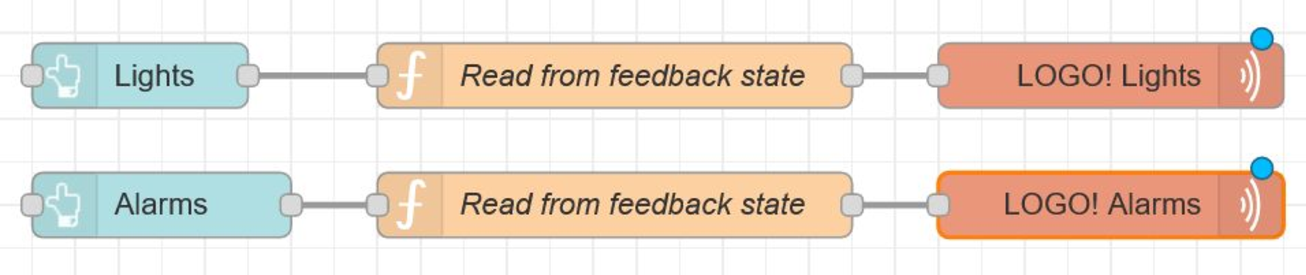
\includegraphics[width=\linewidth]{nodered-app.pdf}
	\caption{Example of WEB-SCADA application created by the author.}
	\label{fig:nodered-app}
\end{figure}


\section{Communication layout}


Overall CR layout is presented in figure \ref{fig:cr-network-topology} and table \ref{tab:cr-element-com}. CR utilizes two main industrial protocols Modbus and S7comm. The author uses Modbus as it is commonly seen in different IACS networks. Thus, Modbus is applied to represent a realistic communication network. S7comm usage is bound to Siemens equipment as most of the Siemens components can communicate using S7comm protocol. Further, both of these protocols are described in detail.


\begin{longtable}[c]{|c|p{0.15\textwidth}|p{0.15\textwidth}|p{0.15\textwidth}|p{0.37\textwidth}|}
	\caption{\raggedright{Communication partners and services running on IACS elements.}}
	\label{tab:cr-element-com}\\
	\hline
	\textbf{Nr.} & \textbf{Component} & \textbf{Interaction partner}     & \textbf{Protocol support} & \textbf{Running processes}                                 \\ \hline
	\endhead
	%
	1            & SCADA              & WEB-SCADA                        & S7comm, FTP               & WinCC advanced V15.1, TIAportal advanced 15.1, FTP server \\ \hline
	2            & WEB-SCADA          & PLC S7-1200, office workstations & Modbus, HTTP, SSH         & Web server, NodeRed, SSH client                           \\ \hline
	3            & PLC LOGO! 8.2      & PLC S7-1200, WEB-SCADA           & S7comm, Modbus            & Warehouse light and alarm control logic and I/O control   \\ \hline
	4            & PLC S7-1200        & SCADA, WEB-SCADA                 & S7comm, Modbus            & Heating plant automation, heating plant HIL simulation    \\ \hline
\end{longtable}


\subsection{Modbus protocol}

All of the detailed and official technical information about Modbus protocol is described in documents \parencite{WEB-21-modbus-main-page, WEB-22-modbus-rfc-doc}. Further, the author highlights particular Modbus technical aspects relevant for this CR, as well as conducted attacks in section \ref{sec:attack-execution}

\begin{figure}[H]
	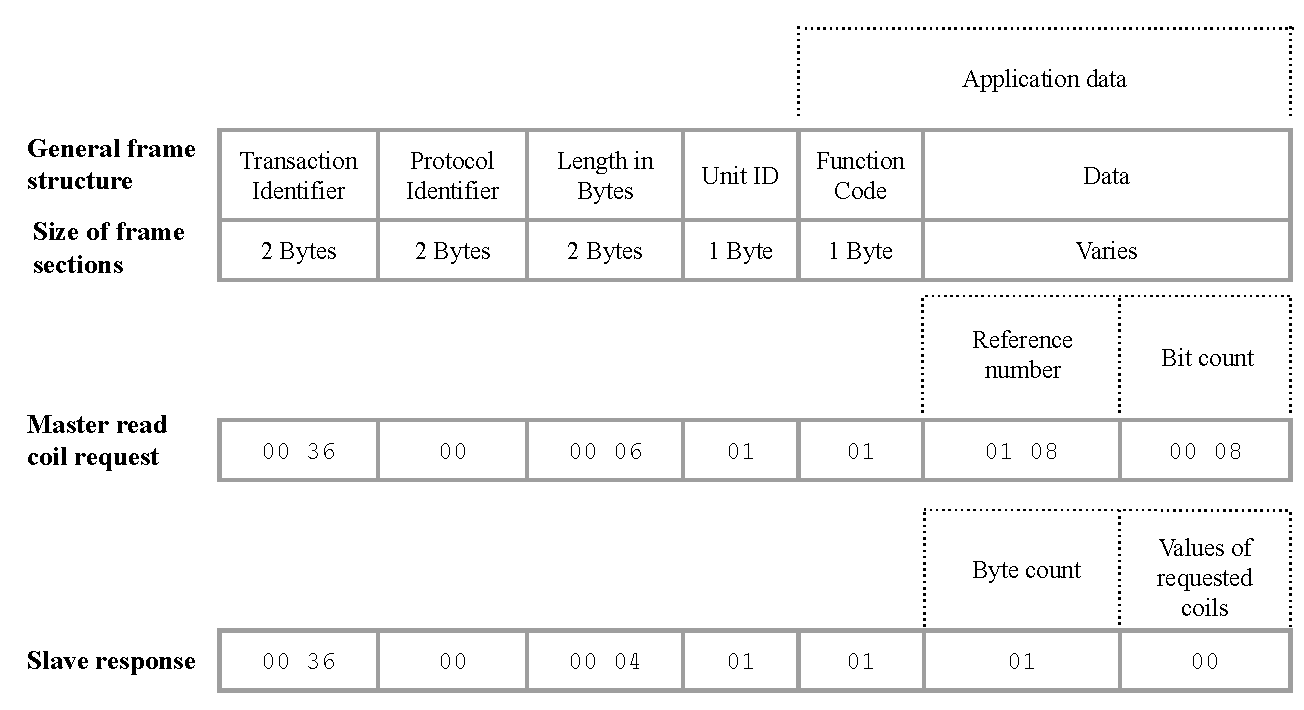
\includegraphics[width=\linewidth]{modbus-frame.pdf}
	\caption{Modbus general frame with examples for master and slave communication frames \parencite{WEB-21-modbus-main-page, WEB-22-modbus-rfc-doc}. Example frames are displayed in hexadecimal.}
	\label{fig:modbus-frame}
\end{figure}

Documentation \parencite{WEB-21-modbus-main-page, WEB-22-modbus-rfc-doc} mentions that Modbus is an open-source protocol developed in the year 1979 for serial communication. Initially, Modbus was used to work with serial communication, but with TCP/IP introduction in the IACS field, Modbus was adopted to work in the TCP/IP stack. Modbus/TCP has become the industry standard for transferring digital and analog I/O information. The protocol's simple implementation made it highly utilized in the IACS environment. Protocol communicates using master (client) and slave (server) architecture. The slave is usually a field-level device like PLC, RTU, or similar device controlling physical processes. Modbus/ TCP embeds a serial Modbus data frame into a TCP/IP frame. A typical master message will consist of function code, determining what action is required from the slave, and required data that depends on the function. Successful slave response includes function code and corresponding data. Function code contains a function number that is standardized but also can be created by a user. Almost all of the devices support six function codes shown in table \ref{tab:modbus-function-codes}.  Examples of Modbus frames in successful communication between devices are displayed in figure \ref{fig:modbus-frame}. If function code is to write or read data from a device, then the data section frame includes memory address or range of addresses. Modbus addresses are mapped to the device memory.

Modbus protocol contains various vulnerabilities such as lack of confidentiality, integrity, and authentication. Relevant vulnerabilities are described in the next chapter \ref{ch:attack-design}

\begin{longtable}[c]{|c|l|p{0.5\textwidth}|}
	
	\caption{\raggedright{Some of the standard Modbus function codes \parencite{WEB-22-modbus-rfc-doc}.}}
	\label{tab:modbus-function-codes}\\
	\hline
	\textbf{Code in hex} & \textbf{Function name}  & \textbf{Description}                                                                          \\ \hline
	\endfirsthead
	\hline
	\textbf{Code in hex} & \textbf{Function name}  & \textbf{Description}                                                                          \\ \hline
	\endhead
	%
	0x01                 & Read coil status        & Reads 1 bit from memory space of the device. used for reading digital output state of the PLC \\ \hline
	0x03                 & Read holding registers  & Reads 2 bytes from memory space of the device. Used for retrieving analog inputs of the PLC   \\ \hline
	0x04                 & Reading input registers & Reads 1 bit from the device. Used to retrieve data about input state of PLC                   \\ \hline
	0x05                 & Force single coil       & Writes 1 bit to the memory of slave.                                                              \\ \hline
	0x0F                 & Force multiple coils    & Writes multiple 1bit values to the slave memory.                                             \\ \hline
	
\end{longtable}



\subsection{S7comm protocol}

S7comm protocol is Siemens proprietary protocol, meaning it does not have detailed official documentation. However, as it is popular, it has been reverse-engineered and thoroughly described in different documents and researches \parencite{WEB-12-wshark-s7comm, WEB-13-s7comm-blog-explained, WEB-23-s7comm-blog-part2, 56-Rogue7-Attacks-On-S7-Simatic-PLC, WEB-24-snap7-documentation-s7comm}. Further, the author highlights particular S7comm technical aspects relevant for this CR, as well as conducted attacks in section \ref{sec:attack-execution}


Summarizing relevant information from \parencite{WEB-12-wshark-s7comm, WEB-13-s7comm-blog-explained, WEB-23-s7comm-blog-part2, 56-Rogue7-Attacks-On-S7-Simatic-PLC, WEB-24-snap7-documentation-s7comm}, S7comm protocol or also called Step7, is an industrial protocol created by Siemens based on ISO 8073 \parencite{WEB-29-s7comm-wireshark} protocol. S7comm protocol is a standard for communicating and programming all Siemens S7 PLCs. This protocol is also utilized for Siemens HMI and SCADA communication. The S7comm is based on TCP/IP, but lacks encryption and authorization. Therefore, it is relatively easy to inject rogue commands into the target. Like Modbus, this protocol works using the master-slave model. This protocol is function-oriented, where master transmission consists of requests. S7comm \gls*{pdu} is encapsulated in TPKT and ISO 8073 \parencite{WEB-29-s7comm-wireshark} protocols and is presented in figure \ref{fig:s7-protocol-owerview}.  To exploit the protocol, PDU is the part attacker manipulates. The header contains length information, PDU reference, and message type. Parameters contain function code and function code related information. Data is an optional field required by some function codes. Step7 closely relies upon the PLC program architecture. The protocol requires to specify \gls*{db} or \gls*{fb} and tags to modify them. For some PLCs, S7comm can update not just only tag values but also the whole PLC program. For an attacker to exploit this protocol library, Snap7 \parencite{WEB-24-snap7-documentation-s7comm} is used since the most important protocol functionality is included in this library.

This protocol has a updated version called S7commPlus, which encrypts the data, increasing security. Research \parencite{101-s7comm-plus-breaking} describes that the S7commPlus encryption can be broken. However, S7commPlus protocol is not in the scope of this research as IACS elements used in this CR cannot fully support this protocol \parencite{WEB-12-wshark-s7comm, WEB-13-s7comm-blog-explained, 83-exploit-siemens-s7}.

\begin{figure}
	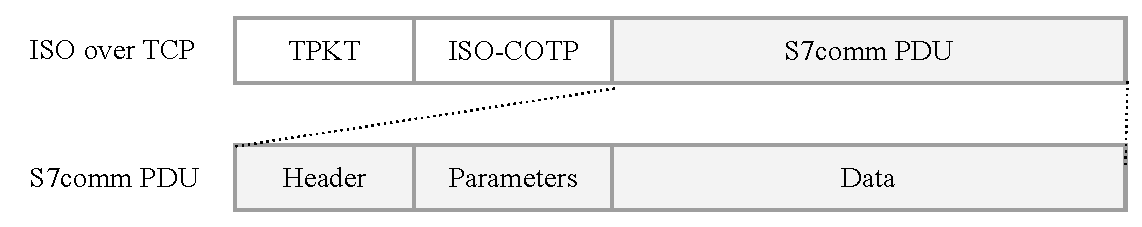
\includegraphics[width=\linewidth]{s7-protocol-owerview.pdf}
	\caption{S7comm protocol frame \parencite{WEB-13-s7comm-blog-explained, WEB-23-s7comm-blog-part2}.}
	\label{fig:s7-protocol-owerview}
\end{figure}
